\documentclass{standalone}

\usepackage{tikz}
\usetikzlibrary{arrows}
\usetikzlibrary{decorations.markings}
\usepackage{standalone}

\begin{document}

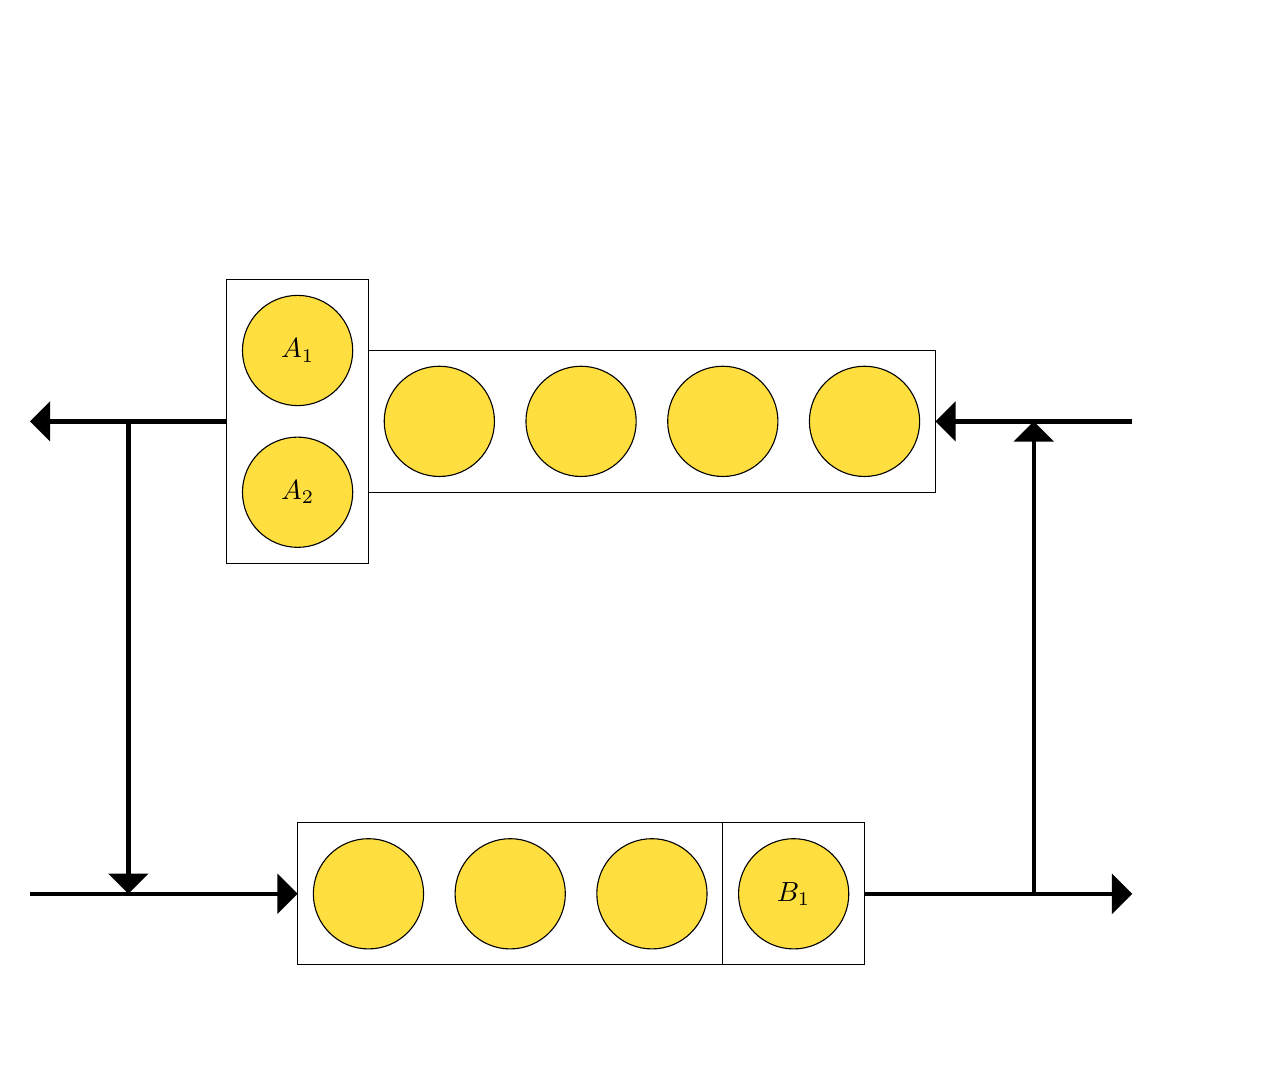
\begin{tikzpicture}

\draw[draw=none] (1, 1) rectangle (16, 14);



% Node bottom
\draw (3.9, 2.1) rectangle (9.3, 3.9);
\draw (9.3, 2.1) rectangle (11.1, 3.9);

% Node middle
\draw (4.8, 8.1) rectangle (12, 9.9);
\draw (3, 7.2) rectangle (4.8, 10.8);



\draw[ultra thick, -triangle 90] (14.5, 9) -- (12, 9); % In to top
\draw[ultra thick, -triangle 90] (3, 9) -- (0.5, 9); % Out of top

\draw[ultra thick, -triangle 90] (0.5, 3) -- (3.9, 3); % In to bottom
\draw[ultra thick, -triangle 90] (11.1, 3) -- (14.5, 3); % Out of bottom

\draw[ultra thick, -triangle 90] (1.75, 9) -- (1.75, 3); % middle to bottom

\draw[ultra thick, -triangle 90] (13.25, 3) -- (13.25, 9); % bottom to middle


% Bottom customers
\node[align=center] [style={minimum size=1.4cm, text width=1.0cm, draw=black,fill={rgb:yellow,4;orange,2;white,2},text=black,shape=circle}] at (3.9, 9.9) {$A_1$};
\node[align=center] [style={minimum size=1.4cm, text width=1.0cm, draw=black,fill={rgb:yellow,4;orange,2;white,2},text=black,shape=circle}] at (3.9, 8.1) {$A_2$};
\node[align=center] [style={minimum size=1.4cm, text width=1.0cm, draw=black,fill={rgb:yellow,4;orange,2;white,2},text=black,shape=circle}] at (5.7, 9) {};
\node[align=center] [style={minimum size=1.4cm, text width=1.0cm, draw=black,fill={rgb:yellow,4;orange,2;white,2},text=black,shape=circle}] at (7.5, 9) {};
\node[align=center] [style={minimum size=1.4cm, text width=1.0cm, draw=black,fill={rgb:yellow,4;orange,2;white,2},text=black,shape=circle}] at (9.3, 9) {};
\node[align=center] [style={minimum size=1.4cm, text width=1.0cm, draw=black,fill={rgb:yellow,4;orange,2;white,2},text=black,shape=circle}] at (11.1, 9) {};

% Bottom customers
\node[align=center] [style={minimum size=1.4cm, text width=1.0cm, draw=black,fill={rgb:yellow,4;orange,2;white,2},text=black,shape=circle}] at (10.2, 3) {$B_1$};
\node[align=center] [style={minimum size=1.4cm, text width=1.0cm, draw=black,fill={rgb:yellow,4;orange,2;white,2},text=black,shape=circle}] at (4.8, 3) {};
\node[align=center] [style={minimum size=1.4cm, text width=1.0cm, draw=black,fill={rgb:yellow,4;orange,2;white,2},text=black,shape=circle}] at (6.6, 3) {};
\node[align=center] [style={minimum size=1.4cm, text width=1.0cm, draw=black,fill={rgb:yellow,4;orange,2;white,2},text=black,shape=circle}] at (8.4, 3) {};


% % B1 to B
% \node[align=center] [style={minimum size=1.4cm, text width=1.0cm, draw=black,fill={rgb:yellow,2;orange,4},text=black,shape=circle}] at (3.9, 9.9) {$A_1$};
% \draw[gray, dashed, ->] (2.8, 9.9) [out=135, in=45, looseness=1.2] to (12.7, 9.5);


% % C1 to B
% \node[align=center] [style={minimum size=1.4cm, text width=1.0cm, draw=black,fill={rgb:yellow,2;orange,4},text=black,shape=circle}] at (10.2, 3) {$B_1$};
% \draw[gray, dashed, ->] (10.9, 3) [bend right=45] to (12.7, 8.5);


% % B2 to C
% \node[align=center] [style={minimum size=1.4cm, text width=1.0cm, draw=black,fill={rgb:yellow,2;orange,4},text=black,shape=circle}] at (3.9, 8.1) {$A_2$};
% \draw[gray, dashed, ->] (3.2, 8.1) [bend right=45] to (3.3, 3.5);





\end{tikzpicture}

\end{document}
